\documentclass[10pt,aps,pra,twocolumn,nofootinbib,superscriptaddress,floatfix]{revtex4-2}
\usepackage[tbtags]{mathtools}
\usepackage{graphicx}
\graphicspath{{figures}}
\usepackage[protrusion,expansion,tracking,kerning,spacing]{microtype}
\usepackage{physics}
\usepackage[final,pdfencoding=auto,hidelinks,colorlinks=true,
  linkcolor=blue,
  filecolor=blue,
  citecolor = black,
urlcolor=cyan]{hyperref} % load late
\usepackage[capitalize]{cleveref}
\usepackage[margin=true,draft]{fixme}
\usepackage{xstring}
\usepackage{natbib}
\usepackage[upint]{stix2}
\usepackage{siunitx}
\usepackage{xcolor}
\usepackage{mathdots}
\usepackage{aligned-overset}
\usepackage{makecell}
\usepackage{cancel} %allows us to strike out text in equations
\usepackage{poormanssubfig}
\usepackage{commonmacros}
\usepackage[RPvoltages, siunitx]{circuitikz}
\crefname{subfigure}{Fig.}{Figs.}

% \label{eq:34}
%% Open Systems
\def\sys{\ensuremath{\mathrm{S}}}
\def\bath{\ensuremath{\mathrm{B}}}
\def\experimental{\ensuremath{\mathrm{exp}}}
\def\inter{\ensuremath{\mathrm{I}}}
\def\drive{\ensuremath{\mathrm{D}}}
\def\cavy{\ensuremath{\mathrm{C}}}
\def\lamb{\ensuremath{\Delta_{\mathrm{L}}}}

%% abs squared
\newcommand{\abss}[1]{\abs{#1}^{2}}

%% polylog
\DeclareMathOperator{\polylog}{polylog}
\DeclareMathOperator{\powerlaw}{powerlaw}

%% io
\newcommand{\inputf}[0]{\ensuremath{\mathrm{in}}}
\newcommand{\outputf}[0]{\ensuremath{\mathrm{out}}}

%% various hamiltonians
\newcommand{\hinter}[2][]{\ensuremath{\widetilde{H}^{I,\infty}_{#1}\pqty{#2}}}

%% pebar
\newcommand{\peb}[0]{\ensuremath{\overline{p_{e}}}}
\newcommand{\esk}[0]{\ensuremath{\overline{\varepsilon}}}

% citation stuff
\newcommand{\refcite}[2][]{{\IfSubStr{#2}{,}{Refs.}{Ref.}~\onlinecite[#1]{#2}}}
\makeatletter
\let\oldbibitem\bibitem
\renewcommand{\bibitem}[2][]{%
  \oldbibitem[#1]{#2}\IfFileExists{{./ref_pdfs/#2.pdf}}{\href{./ref_pdfs/#2.pdf}{[PDF]}~}{}
}
\makeatother

%% Fix hat, tilde
\let\orghat\hat
\def\hat#1{\orghat{\kern0pt #1}}

%% Double braket
\DeclarePairedDelimiter{\Bra}{\lAngle}{\rVert}
\DeclarePairedDelimiter{\Ket}{\lVert}{\rAngle}

\crefname{section}{Sec.}{Secs.}

%% Corrections
\newcommand{\strike}[1]{\textcolor{gray}{#1}}

\usepackage[calc,showseconds=false]{datetime2}

\csname endofdump\endcsname

\usepackage[draft]{conversationalcomments}
\setreviewmarginwidth{1.5in}

% Register Conversation Partners
\usepackage{xcolor}
\definecolor{pastelblue}{RGB}{100, 140, 255}
\definecolor{pastelred}{RGB}{255, 100, 100}
\definecolor{pastelgreen}{RGB}{100, 200, 100}
\newcommentator{icaopo}{Iacopo}{pastelblue}[vale]
\newcommentator{vale}{Vale}{pastelblue}[iacopo]

\raggedbottom

\begin{document}
\synctex=1
\title{Fun with metronomes}

\author{Valentin Boettcher}
\email[]{valentin@physics.mcgill.ca}
\affiliation{McGill University}

\date{\today}
% \begin{abstract}
% \end{abstract}
% \thispagestyle{empty}
% \section*{Current Conversations}

% \subsection*{To Review}
% \printconversations[to-review]{}

% \subsection*{Unresolved}
% \printconversations{}
% \bigskip
% \hrule
% \setcounter{page}{0}
% \clearpage
\maketitle

\section{Introduction}
\label{sec:introduction}

\begin{figure}[ht]
  \centering
  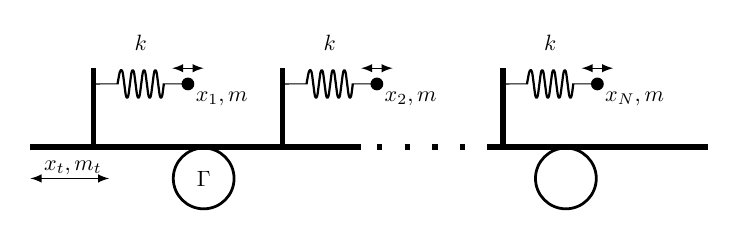
\begin{tikzpicture}[transform shape,scale=.8]
    % Paths, nodes and wires:
    \draw[line width=2pt] (0, 1) -| (5.25, 1);
    \draw[line width=2pt] (1, 1) -- (1, 2.25);
    \draw (1, 2) to[spring, l={$k$}] (2.5, 2);
    \node[circ, xscale=1.65, yscale=1.65](N1) at (2.5, 2){} node[anchor=north west] at (N1.text){$x_1,m$};
    \node[shape=rectangle, minimum width=0.465cm, minimum height=0.465cm] at (0.25, 0.75){} node[anchor=north west, align=left, text width=0.077cm, inner sep=6pt] at (-0, 1){$x_t,m_t$};
    \node[shape=circle, draw, line width=1pt, minimum width=0.965cm](N2) at (2.75, 0.5){} node[anchor=center] at (N2.text){$\Gamma$};
    \node[shape=circle, draw, line width=1pt, minimum width=0.965cm] at (8.5, 0.5){};
    \draw[latex-latex] (0, 0.5) -- (1.25, 0.5);
    \draw[latex-latex] (2.25, 2.25) -- (2.75, 2.25);
    \draw[line width=2pt] (4, 1) -- (4, 2.25);
    \draw (4, 2) to[spring, l={$k$}] (5.5, 2);
    \node[circ, xscale=1.65, yscale=1.65](N3) at (5.5, 2){} node[anchor=north west] at (N3.text){$x_2,m$};
    \draw[latex-latex] (5.25, 2.25) -- (5.75, 2.25);
    \draw[line width=2pt, dash pattern={on 2pt off 8pt}] (5.5, 1) -- (7.25, 1);
    \draw[line width=2pt] (7.25, 1) -- (10.75, 1);
    \draw[line width=2pt] (7.5, 1) -- (7.5, 2.25);
    \draw (7.5, 2) to[spring, l={$k$}] (9, 2);
    \node[circ, xscale=1.65, yscale=1.65](N4) at (9, 2){} node[anchor=north west] at (N4.text){$x_N,m$};
    \draw[latex-latex] (8.75, 2.25) -- (9.25, 2.25);
  \end{tikzpicture}
  \caption{A moving tray with identical masses on identical springs attached}
  \label{fig:tray}
\end{figure}

We begin by deriving the equations of motion for the undampened and undriven setup illustrated in \cref{fig:tray} and will later add damping and drives ad-hoc. The Lagrangian of the above setup is given in terms of the elongation of the masses on the springs \(x_{n}\) relative to their rest position and the position of the tray \(x_{t}\)
\begin{equation}
  \label{eq:1}
  L = T-V = \frac{m_{t}}{2} \dot{x}^{2}_{t}
  + \frac{m}{2}\sum_{n=1}^{N} \dot{x}^{2}_{n} - \frac{k}{2}\sum_{n=1}^{N} x_{n}^{2}.
\end{equation}
The resulting equations of motion with the ad-hoc damping and driving terms (in grey) are
\begin{align}
  \label{eq:3}
  \ddot{x}_{t} + \frac{m}{M} \sum_{n}\ddot{x}_{n}&=  \color{gray}{- \frac{\Gamma}{m_{t}} \dot{x}}\\
  \label{eq:4}\ddot{x}_{n}+\ddot{x}_{t} &= -\frac{k}{m} x_{n} +\color{gray}{\mu \pqty{\hat{x}^{2}-x_{n}^{2}}\dot{x}_{n}},
\end{align}
where \(M= m_{t}+N m\) is the total mass of the system and \(\Gamma\) is the friction coefficient of the tray wheels.
In \cref{eq:4} we also added a \emph{van der Pol} oscillator inspired driving term where \(\mu\) is the drive strength, and \(\hat{x}\) is the ``target amplitude''. Intuitively, the drive tries to keep the maximal oscillator amplitude (and thus its energy) constant just as the wound spring in a metronome\vale{}{Not sure if this is the best model... but including also the kinetic energy in the drive term would be pretty rough.}.

Now inspecting \cref{eq:3} we see that \(x_{t}\) only couples to the collective ``center of mass'' of the spring masses. It is thus useful to Fourier transform the spring elongations:
\begin{equation}
  \label{eq:5}
  y_{k} = \frac{1}{N}\sum_{n} \eu^{-2\pi\iu k n}x_{n}
\end{equation}
where \(k=-\lceil (N-1) / 2\rceil,\ldots,\lfloor(N-1) / 2\rfloor\) and \(y_{-k}=y^{*}_{k}\).

In this ``momentum'' basis,
\begin{align}
  \label{eq:6}
  \ddot{x}_{t} + \frac{m N}{M} \ddot{y}_{0}&=  {- \frac{\Gamma}{m_{t}} \dot{x}_{t}}\\
  \label{eq:7}\ddot{y}_{k}+\delta_{k,0}\ddot{x}_{t} &= -\frac{k}{m} y_{k} +{\frac{\mu}{m} \pqty{\hat{x}^{2}\dot{y}_{k}-\sum_{pq}y_{p}y_{q}\dot{y}_{k-(p+q)}}}.
\end{align}
Albeit the drive term has been much complicated it is now clear that only the common \(y_{0}\) mode couples to the movement of the tray. Setting \(\Gamma=m_{t}=0\) we have
\begin{equation}
  \label{eq:8}
  m {\pqty{\ddot{y}_{0}-\ddot{x_{t}}}} = \underbrace{m \pqty{1 - \frac{mN}{m_{t} + mN}}}_{m_{\text{eff}}}\ddot{y}_{0}=-k y_{k}.
\end{equation}
Low and behold, the \(y_{0}\) mode behaves like an oscillator with an effectively reduced mass. For \(m N \gg m_{t}\) this mass becomes very small \(m_{\text{eff}} \ll m\) and we can expect this mode to react to the drive term more quickly than the other momentum modes. For finite damping \(\Gamma >0\) the tray acceleration \(\ddot{x}_{t}\) will lag behind \(-\ddot{y}_{0}\) reducing the effective mass-reduction and leading to energy loss out of the \(y_{0}\) mode. Thus  without a drive, the \(y_{0}\) mode will always tend to zero at large times while the other modes persist if initially excited.

Initializing the system with \(x_{t}=y_{k}=0\) and random nudges \(\dot{y}_{k}\neq 0\) and assuming that \(\Gamma\) is sufficiently small we see that for short times where \(y_{k}\approx 0\) we can neglect the quadratic terms in the drive to arrive at
\begin{align}
  \label{eq:9}
  \ddot{y}_{0} &= -\frac{k}{m_{\text{eff}}}y_{0} + \frac{\mu}{m_{\text{eff}}}\hat{x}^{2} \dot{y}_{0}\\
  \ddot{y}_{k\neq 0} &= -\frac{k}{m} y_{k} + \frac{\mu}{m}\hat{x}^{2} \dot{y}_{0}
\end{align}
For short times up to order \(t^{2}\) and \(\dot{y}_{0}(0)\neq 0\) we then have
\begin{equation}
  \label{eq:10}
  \frac{{y_{0}(t)}}{y_{k\neq 0}(t)} =
  \frac{m}{m_{\text{eff}}}\frac{{\dot{y}_{0}(0)}}{{\dot{y}_{k}(0)}} \frac{2m_{\text{eff}} +\mu\hat{x}^{2}t }{2m +\mu\hat{x}^{2}t } \overset{t\gtrsim \frac{2m}{\mu \hat{x}^{2}}}{\gg} 1.
\end{equation}
Note that the next term in the short-time expansion of \(y_{k}(t)\) is
\begin{equation}
  \label{eq:11}
  \frac{\hat{x}^{2}\mu^{2}-km_{k}}{6m^{2}_{k}}t^{3
  } \dot{y}_{n}(0),
\end{equation}
where \(m_{0}=m_{\text{eff}}\) and \(m_{k\neq 0}=m\).  Therefore we can expect that for \(\hat{x}^{2}\mu^{2} \gg k m_{\text{eff}}\) the \(k=0\) mode remains strongly favored. Conversely, if \(\mu\) or \(\hat{x}\) is to small, we can expect the \(k=0\) mode to have to compete with the other modes.
Extrapolating this argument provides a heuristic explanation of why the \(k=0\) mode is preferred and the oscillators synchronize.

For negligible damping and setting \(y_{k\neq0}=0\) the equation of motion for \(y_{0}\)  from \cref{eq:7} then becomes
\begin{equation}
  \label{eq:14}
  \ddot{y}_{0} = -\frac{k}{m_{\text{eff}}}y_{0} + \frac{{\mu}}{m_{\text{eff}}}\bqty{\hat{x}^{2}- y_{0}^{2}}\dot{y}_{0}
\end{equation}
which is a single van der Pol oscillator~\cite{Strogatz2018}.
The van der Pol oscillator has a stable limit cycle for all parameter values (although it may be reached more slowly for some regimes).
Mapping to the standard dimensionless form of the equation we have\vale{}{I should probably make all equations dimensionless.}
\begin{equation}
  \label{eq:16}
  \ddot{\chi} = -\chi + \tilde{\mu} \pqty{1-\chi^{2}}\dot{\chi},
\end{equation}
where we transformed \(t\to \tau = \omega_{0}t\) (with \(\omega_{0}=\sqrt{ k /m_{\text{eff}}}\)), \(y_{0}(t)\to \hat{x} \chi(\tau)\), and
\begin{equation}
  \label{eq:2}
  \tilde{\mu} =\frac{\mu \hat{x}^{2}}{m \omega_{0}} = \frac{\mu\hat{x}^{2}}{\sqrt{km}} .
\end{equation}

For \(\tilde{\mu}\ll1\) the approximate solution of \cref{eq:12} is~\cite{Strogatz2018}
\begin{equation}
  \label{eq:15}
  y_{0}(t) \approx 2 \hat{x} \sin(\omega_{0}t).
\end{equation}
For large \({\mu} / ({m_{\text{eff}}}\omega_{0}) \) the limit cycle that is reached reached into on time scales of order \({1} / {\tilde{\mu} \omega_{0}}\) still has the approximate amplitude \(2\hat{x}\) but with a non-sinusoidal shape a period of
\begin{equation}
  \label{eq:17}
  T = \frac{\tilde{\mu}}{\omega_{0}} = \frac{\mu\hat{x}^{2}}{k}.
\end{equation}

However, this regime is characterized by long dwell times at maximum (minimum) elongation and rapid transitions which does not resemble the movement of a metronome.
The mean square displacement of \(y_{0}\) ranges between the two extremes at \(\tilde{\mu} \ll 1\) and \(\tilde{\mu}\)
\begin{equation}
  \label{eq:18}
  2\hat{x}^{2}\lesssim \ev{y_{0}^{2}} \lesssim 4\hat{x}^{2}.
\end{equation}

To probe the stability of the synchronized mode \(y_{k}\) add a small perturbation \(y_{k\neq0} = \delta y\) with \(\delta y(0) \ll \max_{t} \abs{y_{0}(t) \approx 2x}\).
We now assume that the limit-cycle period of \(y_{0}\) is sufficiently short compared so that. Then, we can drop zero-mean fast-oscillating proportional to \(y_{0}(t)\) and \(y(t)\) and find from \cref{eq:7}
\begin{equation}
  \label{eq:12}
  \delta\ddot{y}
  \approx-\frac{k}{m} y +\mu \bqty{\hat{x}^{2} - \Bqty{3+(N-3)N}y^{2} - \ev{y_{0}^{2}} }\delta\dot{y}
\end{equation}
The coefficient of the drive term is negative thus induces damping and stabilizes the \(y_{0}\) mode for
\begin{equation}
  \label{eq:13}
  \hat{x}^{2} < \bqty{3+(N-3)N} y^{2} +\ev{y_{0}^{2}}.
\end{equation}
This condition is fulfilled either if \(N\) is sufficiently large, or \(y_0\) has successfully locked into its limit cycle (see \cref{eq:17}).

I suspect therefore the criteria for a stable synchronization of metronomes to be:
\begin{enumerate}
  \item small tray mass \(m_{t}\ll m N\) and low friction
  \item \(\delta y \ll \hat{x}\): in order that the approximation works
  \item \(\tilde{\mu}\):
    \begin{itemize}
      \item too large values: non-metronome like movement
      \item too small values: slow damping of perturbations (\cref{eq:12}) and slow promotion of \(y_{0}\) mode (see \cref{eq:10})
    \end{itemize}
\end{enumerate}

Conversely, the synchronization phenomenon can be destroyed by having a heavy tray and large friction.
\clearpage
\bibliography{references}
\end{document}

%%% Local Variables:
%%% mode: latex/mps
%%% TeX-master: t
%%% TeX-output-dir: "output"
%%% TeX-engine: default
%%% jinx-languages: "en_US"
%%% End:
